\chapter{Quantum Algorithms}
Quantum computers promise to solve problems intractable by classical computers. One application is quantum simulation. For example: simulating chemical processes, which are actually quantum processes. As Richard Feynman said: \say{\emph{Nature isn't classical, dammit, and if you want to make a simulation of nature, you'd better make it quantum mechanical.}} Other possible applications include optimization, cryptography and machine learning. There are a lot of efforts in trying to apply quantum computing, but many remain skeptic. We should assume no guarantees in the applications of quantum computers, but continue exploring the possibilities.

When a quantum computer can calculate something efficiently that a classical computer cannot calculate efficiently, we will have reached \emph{quantum supremacy}. The boundary of reaching this is around 50 qubits, when it becomes impossible to simulate a quantum computer. We have not yet reached quantum supremacy, but we are getting close to it. There have been found quantum algorithms which provide a speedup over classical algorithms, like Shor's algorithm for factoring integers and the Deutch-Jozsa algorithm for determining if a boolean function is balanced or unbalanced.

\section{Quantum Arithmetic}
Any classical circuit can be simulated by a quantum circuit. We can show this by creating quantum versions of classical arithmetic functions. One problem with simulating classical gates as quantum gates is that most of them are non-reversible. In quantum computing, it is required for gates to be reversible. This is often solved by adding an output qubit for every input qubit and an extra result qubit (Figure~\ref{fig:add_output_qubit}).
\begin{figure}[ht]
  \[
    \Large
    \Qcircuit @C=1em @R=0.5em {
      \push{\rule{0em}{1em}} & & \lstick{\ket{x}} & \multigate{1}{U_f} & \qw & \ket{x} \\
      \push{\rule{0em}{1em}} & & \lstick{\ket{y}} & \ghost{U_f} & \qw & & \hspace*{5.7mm} \ket{y \oplus f(x)}
    }
  \]
  \caption{Create output qubits for every input qubit in \ket{x} and store the result of $f(x)$ in \ket{y}. This transformation can be described as $U_f\ket{x}\!\ket{y} = \ket{x}\!\ket{y \oplus f(x)}$. The $\oplus$ symbol in this context means the binary sum (\textsc{xor}).}
  \label{fig:add_output_qubit}
\end{figure}
We can create a quantum half adder by creating sum and carry circuits, just like in classical computers. The truth table of the sum function $f_s(x)$ can be found in Figure \ref{fig:sum_truth_table}. We can implement this as a quantum circuit using \textsc{cnot} gates as seen in Figure \ref{fig:sum_quantum_circuit}.

\begin{figure}[ht]
  \begin{minipage}{.45\textwidth}
    \centering
    \begin{tabular}{c|c}
      $x_0$$x_1$ & $f_s(x)$ \\ \hline
      00 & 0 \\
      01 & 1 \\
      10 & 1 \\
      11 & 0 \\
    \end{tabular}
    \caption{Bit sum truth table.}
    \label{fig:sum_truth_table}
  \end{minipage}%
  \hspace*{.05\textwidth}
  \begin{minipage}{.45\textwidth}
    \[
      \Large
      \Qcircuit @C=1em @R=0.5em @!R {
        \push{\rule{0em}{1em}} & & \lstick{\ket{x_{0}}} & \ctrl{2} & \qw & \qw \\
        \push{\rule{0em}{1em}} & & \lstick{\ket{x_{1}}} & \qw & \ctrl{1} & \qw \\
        \push{\rule{0em}{1em}} & & \lstick{\ket{y}} & \targ &  \targ & \qw \\
      }
    \]
    \caption{Quantum circuit for summing two bits using two \textsc{cnot} gates.}
    \label{fig:sum_quantum_circuit}
  \end{minipage}
\end{figure}
\newpage

To fully add two bits we need to account for the carry. The carry function $f_c(x)$ is 1 if and only if both inputs are 1 (Figure~\ref{fig:carry_truth_table}). This truth table corresponds directly to the Toffoli gate (Figure~\ref{fig:carry_quantum_circuit}).

\begin{figure}[ht]
  \begin{minipage}{.45\textwidth}
    \centering
    \begin{tabular}{c|c}
      $x_0$$x_1$ & $f_c(x)$ \\ \hline
      00 & 0 \\
      01 & 0 \\
      10 & 0 \\
      11 & 1 \\
    \end{tabular}
    \caption{Bit carry truth table.}
    \label{fig:carry_truth_table}
  \end{minipage}%
  \hspace*{.05\textwidth}
  \begin{minipage}{.45\textwidth}
    \[
      \Large
      \Qcircuit @C=1em @R=0.5em @!R {
        \push{\rule{0em}{1em}} & & \lstick{\ket{x_{0}}} & \ctrl{2} & \qw \\
        \push{\rule{0em}{1em}} & & \lstick{\ket{x_{1}}} & \ctrl{1} & \qw \\
        \push{\rule{0em}{1em}} & & \lstick{\ket{y}} & \targ & \qw \\
      }
    \]
    \caption{Quantum circuit for taking the carry of two bits implemented using a Toffoli gate.}
    \label{fig:carry_quantum_circuit}
  \end{minipage}
\end{figure}
\noindent
We can combine our sum and carry circuit into one, creating a quantum half adder.

\begin{figure}[ht]
  \[
    \Large
    \Qcircuit @C=1em @R=0.5em @!R {
      \push{\rule{0em}{1em}} & \lstick{\ket{x_0}} & \ctrl{3} & \ctrl{2} & \qw & \qw & \ket{x_0} \\
      \push{\rule{0em}{1em}} & \lstick{\ket{x_1}} & \ctrl{2} & \qw &  \ctrl{1} & \qw & \ket{x_1} \\
      \push{\rule{0em}{1em}} & \lstick{\ket{0}} & \qw & \targ & \targ & \qw & \ket{y_s} \\
      \push{\rule{0em}{1em}} & \lstick{\ket{0}} & \targ & \qw & \qw & \qw & \ket{y_c} \\
    }
  \]
  \caption{Quantum half adder. The sum ends up in \ket{y_s} and the carry in \ket{y_c}.}
  \label{fig:quantum_full_adder}
\end{figure}

Let's check if this circuit works. Say we want to add $\ket{x_0} = \ket{1}$ and $\ket{x_1} = \ket{1}$. We would expect to get \ket{0} as sum and \ket{1} as carry. Our initial state is \ket{1100}. We apply a Toffoli gate, setting the carry qubit to 1: \ket{1101}. Then we set the sum qubit by doing a $\textsc{cnot}_{0,2}$ and a $\textsc{cnot}_{1,2}$ ending up with the state \ket{1101}. Measuring the sum and carry qubits gives $M(y_s) = \ket{0}$ and $M(y_c) = \ket{1}$, giving us what we expected and thus having done a quantum half addition of two qubits.

\section{Deutch-Jozsa Algorithm}
We have shown that we can simulate classical circuits on a quantum computer. This itself isn't very impressive however, we could already do that on a classical computer. In this section we will describe an algorithm with quantum speedup. Consider the four single-bit operations identity, \textsc{not}, reset and set.

\begin{figure}[ht]
  \centering
  \begin{multicols}{4}
    \captionof*{table}{\textbf{Identity}\\$f_i(x) = x$}
    \begin{tabular}{c|c}
      $x$ & $f_i(x)$ \\ \hline
      0 & 0 \\
      1 & 1 \\
    \end{tabular}

    \captionof*{table}{\textbf{NOT}\\$f_n(x) = \neg x$}
    \begin{tabular}{c|c}
      $x$ & $f_n(x)$ \\ \hline
      0 & 1 \\
      1 & 0 \\
    \end{tabular}

    \captionof*{table}{\textbf{Reset}\\$f_r(x) = 0$}
    \begin{tabular}{c|c}
      $x$ & $f_r(x)$ \\ \hline
      0 & 0 \\
      1 & 0 \\
    \end{tabular}

    \captionof*{table}{\textbf{Set}\\$f_s(x) = 1$}
    \begin{tabular}{c|c}
      $x$ & $f_s(x)$ \\ \hline
      0 & 1 \\
      1 & 1 \\
    \end{tabular}
  \end{multicols}

  \vspace{4mm}
  \caption{Truth tables for the four single-bit operations.}
  \label{fig:single_bit_operations}
\end{figure}
\noindent
Say we are faced with the following problem: we have a ``black box" with one of the four one-bit functions, but we're not told which one. Determine if the function is \emph{balanced} or \emph{unbalanced}. A balanced function is a function which returns the same amount of 0 and 1s it received as input, like identity and \textsc{not}. Unbalanced functions are functions which return a constant value, like reset and set. This is known as \emph{Deutch's problem} and is one of the first examples of a problem where there exists a quantum algorithm that is exponentially faster than any deterministic classical algorithm.

On a classical computer, to determine if the black box is balanced or unbalanced, we need to do two function calls. On a quantum computer, using the \emph{Deutch-Jozsa} algorithm, we can figure it out using one call to the black box. To use this algorithm for Deutch's problem we need to translate the four single-bit operations to the quantum world. The quantum circuits corresponding to each single-bit operation can be found in Figure~\ref{fig:single_bit_quantum_circuits}.
\vspace{-8mm}
\begin{figure}[ht]
  \centering
  \begin{multicols}{4}
    \[
      \Qcircuit @C=0.7em @R=0.8em @!R {
        \push{\rule{0em}{1em}} & & \lstick{\ket{x}} & \ctrl{1} & \qw \\
        \push{\rule{0em}{1em}} & & \lstick{\ket{y}} & \targ & \qw
      }
    \]
    \caption*{\textbf{Identity}\\$f_i(x) = x$}

    \[
      \Qcircuit @C=0.7em @R=0.5em @!R {
        \push{\rule{0em}{1em}} & & \lstick{\ket{x}} & \gate{X} & \ctrl{1} & \gate{X} & \qw \\
        \push{\rule{0em}{1em}} & & \lstick{\ket{y}} & \qw & \targ & \qw & \qw
      }
    \]
    \caption*{\textbf{NOT}\\$f_n(x) = \neg x$}

    \[
      \Qcircuit @C=0.7em @R=0.8em @!R {
        \push{\rule{0em}{1em}} & & & & & \lstick{\ket{x}} & \qw & \qw & \ghost{X} \\
        \push{\rule{0em}{1em}} & & & & & \lstick{\ket{y}} & \qw & \qw & \ghost{X}
      }
    \]
    \caption*{\textbf{Reset}\\$f_r(x) = 0$}

    \[
      \Qcircuit @C=0.7em @R=0.5em @!R {
        \push{\rule{0em}{1em}} & & \lstick{\ket{x}} & \qw & \qw \\
        \push{\rule{0em}{1em}} & & \lstick{\ket{y}} & \gate{X} & \qw
      }
    \]
    \caption*{\textbf{Set}\\$f_s(x) = 1$}
  \end{multicols}

  \vspace{3mm}
  \caption{Quantum circuit representation of the four single-bit operations.}
  \label{fig:single_bit_quantum_circuits}
\end{figure}

\noindent
With these definitions we can start using the Deutch-Jozsa algorithm to efficiently determine what kind of function our black box is. The circuit to do so is described in Figure~\ref{fig:deutch_jozsa_circuit}. In this circuit, $U_f$ refers to our black box function, or as it is sometimes also called, \emph{oracle}.

\begin{figure}[ht]
  \[
    \Large
    \Qcircuit @C=1em @R=1em @!R {
      \push{\rule{0em}{1em}} & & & & \lstick{\ket{x} = \ket{0}} & \gate{H} & \multigate{1}{U_f} & \gate{H} & \meter & \cw \\
      \push{\rule{0em}{1em}} & & & & \lstick{\ket{y} = \ket{1}} & \gate{H} & \ghost{U_f} &  \qw & \qw & \qw
    }
  \]
  \caption{Quantum circuit to determine if $f$ is a balanced or unbalanced function using the Deutch-Jozsa algorithm. $U_f$ is the quantum circuit which transforms \ket{x}\ket{y} to \ket{x}\ket{y \oplus f(x)}.}
  \label{fig:deutch_jozsa_circuit}
\end{figure}
We can try it out by trying to determine if the identity function $f_i(x) = x$ is balanced or unbalanced. We start with putting \ket{x} and \ket{y} through a Hadamard gate:
\begin{equation}
  \ket{\psi} = \dfrac{1}{2}(\ket{00} - \ket{01} + \ket{10} - \ket{11}).
\end{equation}
We evaluate our identity function using by applying $U_f$:
\begin{equation}
  \begin{aligned}
    \ket{\psi} = \dfrac{1}{2}\big(&\ket{0}\!\ket{0 \oplus f_i(0)} - \ket{0}\!\ket{1 \oplus f_i(0)} \\
    +\, &\ket{1}\!\ket{0 \oplus f_i(1)} - \ket{1}\!\ket{1 \oplus f_i(1)}\big).
  \end{aligned}
\end{equation}
This state contains information about both $f_i(0)$ and $f_i(1)$! We have essentially evaluated two values of $f_i(x)$ simultaneously, a feature known as \emph{quantum parallelism}. Actually applying the function $f_i(x)$, which as we can see in Figure~\ref{fig:single_bit_quantum_circuits} is just a $\textsc{cnot}_{0, 1}$, gives us the state
\begin{equation}
  \ket{\psi} = \dfrac{1}{2}(\ket{00} - \ket{01} + \ket{11} - \ket{10}).
\end{equation}
Finally we apply another Hadamard gate on \ket{x}:
\begin{equation}
  \begin{aligned}
    \ket{\psi} = \dfrac{1}{2\sqrt2}(&\ket{00} + \ket{10} - \ket{01} - \ket{11} \\
    + \, &\ket{01} - \ket{11} - \ket{00} + \ket{10})
  \end{aligned}
\end{equation}
\vspace*{-7mm}
\begin{align}
  \phantom{\ket{\psi}} &= \dfrac{1}{2\sqrt2}(\ket{10} + \ket{10} - \ket{11} - \ket{11}) \\
  &= \dfrac{1}{\sqrt2}(\ket{10} - \ket{11}).
\end{align}
We end up with the final state $(\ket{10} - \ket{11})/\sqrt2$ before measurement. We can see from this state that $M(x) = \ket{1}$. Curiously, the following measurement outcomes apply:
\begin{equation}
  \begin{aligned}
    \ket{0_x} \otimes \dfrac{1}{\sqrt2}(\ket{0_y} - \ket{1_y}) & \, \text{ if } \, f(0) = f(1) \\
    \ket{1_x} \otimes \dfrac{1}{\sqrt2}(\ket{0_y} - \ket{1_y}) & \, \text{ if } \, f(0) \not= f(1)
  \end{aligned}
\end{equation}
That is, we get $M(x) = \ket{1}$ if $f(0) \not= f(1)$, which means $f$ is a balanced function. Likewise, we get $M(x) = \ket{0}$ if $f(0) = f(1)$, which means $f$ is an unbalanced function. Since we got a measurement of \ket{1} for $f_i$, and given the fact that the identity operation is balanced, we can say that we effectively determined that $f_i$ is a balanced function with one call to the black box.

\section{Quantum Fourier Transform}
An important operation in classical computing and quantum computing as we will see is the \emph{Fourier transform}. The Fourier transform transforms a function $f(t)$ in the time domain to another function $F(x)$ in the frequency domain. The opposite (transforming a function in the frequency domain to a function in the time domain) can be achieved by applying the \emph{inverse} Fourier transform. Consider the sinusoidal function $\cos(t)$. Figure~\ref{fig:cos_time_graph} graphs this function in the time domain, with time on the $x$ axis and amplitude on the $y$ axis. Applying the Fourier transform on this function gives us a function of the frequency domain, as seen in Figure~\ref{fig:cos_freq_graph}.
\begin{figure}[ht]
  \centering
  \begin{multicols}{2}
    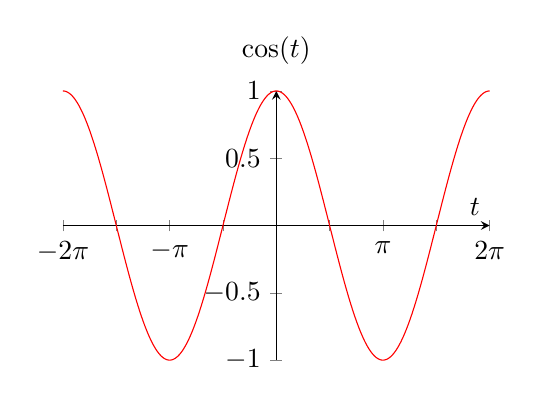
\begin{tikzpicture}
      \begin{axis}[
        title={$\cos(t)$},
        xlabel={$t$},
        axis lines = middle,
        xmax=2*pi,
        xmin=-2*pi,
        height=5cm,
        width=7cm,
        ymin=-1,
        ymax=1,
        xticklabels={$-2\pi$, , $-\pi$, ,
            , $\pi$, , $2\pi$},
        xtick={-6.28318, -4.7123889, -3.14159, -1.5708, 1.5708, 3.14159, 4.7123889, 6.28318}
      ]
        \addplot[red, domain=-2*pi:2*pi, samples=1000]{ cos(deg(x)) };
      \end{axis}
    \end{tikzpicture}
    \caption{Time domain plot of $\cos(t)$.}
    \label{fig:cos_time_graph}

    \begin{tikzpicture}
      \begin{axis}[
        title={$F(\cos(t))$},
        xlabel={$x$},
        axis lines=middle,
        height=5cm,
        width=6cm,
        xmax=2,
        xmin=-2,
        ymin=0,
        ymax=2
       ]
         \addplot[ycomb, blue, mark=, thick, mark=*] coordinates {
           (1, 1) (-1, 1)
         };
      \end{axis}
    \end{tikzpicture}
    \caption{Frequency domain plot of $F(\cos(t))$.}
    \label{fig:cos_freq_graph}
  \end{multicols}
\end{figure}

The Fourier transform is a very useful tool in computer science, used for example in signal processing. The signal shown in Figure~\ref{fig:cos_time_graph} is a continuous signal, meaning it is assumed to extend to infinity. Computers however can only deal with finite, non-continuous signals. This means we have to discretize the continuous function into discrete counterparts as seen in Figure~\ref{fig:cos_discrete_time_graph}. We can then transform the discrete signal using the \emph{discrete Fourier transform}.
\begin{figure}[ht]
  \centering
  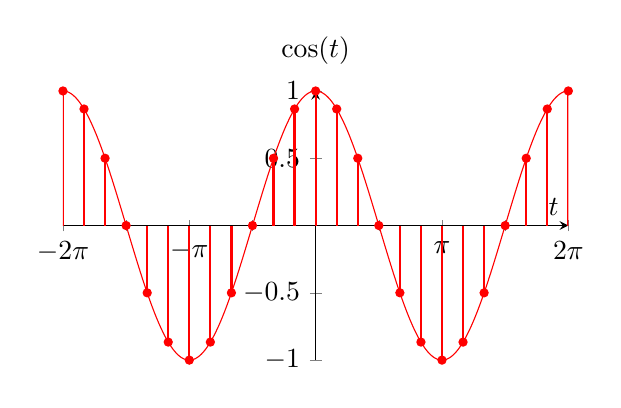
\begin{tikzpicture}
    \begin{axis}[
      title={$\cos(t)$},
      xlabel={$t$},
      axis lines = middle,
      xmax=2*pi,
      xmin=-2*pi,
      height=5cm,
      width=8cm,
      ymin=-1,
      ymax=1,
      xticklabels={$-2\pi$, , $-\pi$, , , $\pi$, , $2\pi$},
      xtick={-6.28318, -4.7123889, -3.14159, -1.5708, 1.5708, 3.14159, 4.7123889, 6.28318}
    ]
      \addplot[ycomb, red, domain=-2*pi:2*pi, samples=25, mark=*, thick, mark size=1.25pt]{ cos(deg(x)) };
      \addplot[red, domain=-2*pi:2*pi, samples=1000, draw]{ cos(deg(x)) };
    \end{axis}
  \end{tikzpicture}
  \caption{Discretized counterpart of the continuous function $\cos(t)$. Each dot represents a sample of the signal. The time between the samples is called the sampling interval.}
  \label{fig:cos_discrete_time_graph}
\end{figure}

The discrete Fourier transform can be thought of as a linear operation. This means we can map a $N$-dimensional state vector to another $N$-dimensional state vector by a $N \times N$ matrix $F_N$. For a $n$ qubit state $N$ is equal to $2^n$. Such transformation may be written as
\begin{equation}
  \ket{x} = \sum_{j=0}^{N-1}x_j\ket{j} \longrightarrow \sum_{k=0}^{N-1}y_k\ket{k},
\end{equation}
where the amplitudes $y_k$ are the discrete Fourier transform of the amplitudes $x_j$. In other words, the quantum Fourier transform (QFT) transforms the computational basis states as following
\begin{equation} \label{eq:qft}
  F_N\ket{j} = \dfrac{1}{\sqrt N}\sum_{k=0}^{N-1}e^{2\pi i jk/N}\ket{k}.
\end{equation}
Note that this is the equivalent of a classical \emph{inverse} discrete Fourier transform. The quantum Fourier transform (QFT) has the same effect as the classical inverse Fourier transform and vice versa. The quantum Fourier transform provides an exponential speedup over the classical fast Fourier transform algorithm.

We have already seen and used the QFT on a single qubit. The unitary matrix of the QFT on one qubit is the Hadamard gate:
\begin{equation}
  F_2 = H = \hgate.
\end{equation}
For a multi-qubit system it becomes a bit more involved. To describe the circuit for the $n$-qubit QFT we need the Hadamard and controlled phase gate. We will write the phase gate as $R_k$ where
\begin{equation}
  R_k = \begin{pmatrix}
    1 & 0 \\
    0 & e^{2\pi i/2^k}
  \end{pmatrix}.
\end{equation}
The circuit for a QFT on 3 qubits can be seen in Figure~\ref{fig:quantum_3_qubit_fourier_circ}. Note that $S = R_2$ and $T = R_3$. The crossed gate at the end is the swap gate, which swaps two qubits. The order of qubits has to be reversed at the end of a QFT to get the correct order as result. Note that inverting the circuit by reversing the order of the gates and taking the inverse $U^\dagger$ of each gate $U$ gives an equally efficient circuit for the inverse quantum Fourier transform $F_N^\dagger$.

\begin{figure}[ht]
  \[
    \Large
    \Qcircuit @C=1em @R=0.5em @!R {
      \push{\rule{0em}{1em}} & & \lstick{\ket{x_0}} & \gate{H} & \gate{S} & \gate{T} & \qw & \qw & \qw & \qswap & \qw \\
      \push{\rule{0em}{1em}} & & \lstick{\ket{x_1}} & \qw & \ctrl{-1} & \qw & \gate{H} & \gate{S} & \qw & \qw \qwx & \qw \\
      \push{\rule{0em}{1em}} & & \lstick{\ket{x_2}} & \qw & \qw & \ctrl{-2} & \qw & \ctrl{-1} & \gate{H} & \qswap \qwx & \qw \\
    }
  \]
  \caption{Quantum Fourier transform on 3 qubits.}
  \label{fig:quantum_3_qubit_fourier_circ}
\end{figure}
\noindent
The matrix of a QFT can be written out using $\omega = e^{2\pi i/N}$. For 3 qubits, where $N = 8$:
\begin{equation}
  F_8 = \dfrac{1}{\sqrt 8}
  \begin{pmatrix}
    1 & 1 & 1 & 1 & 1 & 1 & 1 & 1 \\
    1 & \omega^1 & \omega^2 & \omega^3 & \omega^4 & \omega^5 & \omega^6 & \omega^7 \\
    1 & \omega^2 & \omega^4 & \omega^6 & 1 & \omega^2 & \omega^4 & \omega^6 \\
    1 & \omega^3 & \omega^6 & \omega^1 & \omega^4 & \omega^7 & \omega^2 & \omega^5 \\
    1 & \omega^4 & 1 & \omega^4 & 1 & \omega^4 & 1 & \omega^4 \\
    1 & \omega^5 & \omega^2 & \omega^7 & \omega^4 & \omega^1 & \omega^6 & \omega^3 \\
    1 & \omega^6 & \omega^4 & \omega^2 & 1 & \omega^6 & \omega^4 & \omega^2 \\
    1 & \omega^7 & \omega^6 & \omega^5 & \omega^4 & \omega^3 & \omega^2 & \omega^1 \\
  \end{pmatrix}.
\end{equation}
A more general circuit of the QFT for a $n$ qubit state is described below in Figure~\ref{fig:quantum_fourier_circ}.

\begin{figure}[ht]
  \begin{adjustwidth}{-2.5cm}{-2.5cm}
    \[
      \Qcircuit @C=0.9em @R=0.5em @!R {
        \push{\rule{0em}{1em}} & & \lstick{\ket{x_0}} & \gate{H} & \gate{R_2} & \qw & \dots & & \gate{R_{n-1}} & \gate{R_n} & \qw & \qw & \qw & \qw & \qw & \qw & \qw & \qw & \qw & \qw & \qw & \qw & \qw \\
        \push{\rule{0em}{1em}} & & \lstick{\ket{x_1}} & \qw & \ctrl{-1} & \qw & \dots & & \qw & \qw & \gate{H} & \qw & \dots & & \gate{R_{n-2}} & \gate{R_{n-1}} & \qw & \dots & & \qw & \qw & \qw & \qw \\
        \rstick{\vdots} & & & & \vdots & & & & & & & & & & & \\
        \push{\rule{0em}{1em}} & & \lstick{\ket{x_{n - 1}}} & \qw & \qw & \qw & \qw & \qw & \ctrl{-3} & \qw & \qw & \qw & \qw & \qw & \ctrl{-2} & \qw & \qw & \dots & & \gate{H} & \gate{R_2} & \qw & \qw \\
        \push{\rule{0em}{1em}} & & \lstick{\ket{x_n}} & \qw  & \qw & \qw & \qw & \qw & \qw & \ctrl{-4} & \qw & \qw & \qw & \qw & \qw & \ctrl{-3} & \qw & \dots & & \qw & \ctrl{-1} & \gate{H} & \qw \\
      }
    \]
  \end{adjustwidth}
  \caption{Quantum Fourier transform on $n$ qubits. Swap gates required to get the correct order at the end are omitted.}
  \label{fig:quantum_fourier_circ}
\end{figure}
The result of the Fourier transform of the original state is stored in the amplitudes. Remember however that these amplitudes cannot be extracted. Thus there is no way of determining the Fourier transform of the original state using the QFT\@. Even though we can't extract the transformed values after a QFT, the QFT has its use in quantum algorithms like Shor's algorithm for factoring integers and the quantum phase estimation algorithm.

\newpage

\section{Quantum Phase Estimation Algorithm}
The quantum phase estimation algorithm (QPE) is a quantum algorithm to estimate the phase of an eigenvector of a unitary operation. Say we prepare an eigenstate \ket{u} of a unitary operator $U$, where $U\!\ket{u} = e^{2\pi i \varphi}\ket{u}$ and the value of $\varphi$ is unknown ($0 \le \varphi \le 1$). The goal is to estimate the value of $\varphi$ when we don't necessarily know $U$ or \ket{u}, but have available black boxes capable of preparing \ket{u} and applying controlled-$U$ operations.

\begin{figure}[ht]
  \[
    \Large
    \Qcircuit @C=0.9em @R=0.5em @!R {
      \push{\rule{0em}{1em}} & & \lstick{\ket{0}} & \gate{H} & \qw & \qw & \qw & \dots & & \ctrl{4} & \multigate{3}{\,F^\dagger_n\,} & \qw & \meter & \cw \\
      \rstick{\vdots} & & & \vdots & & & & & & & & & \vdots \\
      \push{\rule{0em}{1em}} & & \lstick{\ket{0}} & \gate{H} & \qw & \ctrl{2} & \qw & \dots & & \qw & \ghost{\,F^\dagger_n\,} & \qw & \meter & \cw \\
      \push{\rule{0em}{1em}} & & \lstick{\ket{0}} & \gate{H} & \ctrl{1} &  \qw & \qw & \dots & & \qw & \ghost{\,F^\dagger_n\,} & \qw & \meter & \cw \\
      \push{\rule{0em}{1em}} & & \lstick{\ket{u}} & \qw {/^m} & \gate{U^{2^0}} & \gate{U^{2^1}} & \qw & \dots & & \gate{U^{2^{n-1}}} & \qw & \qw & \qw & \qw \\
    }
  \]
  \caption{Quantum phase estimation circuit, where $F^\dagger_n$ represent the inverse quantum Fourier transform on $n$ qubits. The ``/" denotes a register of $m$ qubits.}
  \label{fig:phase_estimation_circ}
\end{figure}

The circuit for the QPE algorithm found in Figure~\ref{fig:phase_estimation_circ} consists of two registers. The upper $n$ qubits comprise the first register which will be used to calculate the estimate of $\varphi$. The size of the first register can be chosen based on two factors: accuracy and success probability. More qubits will give you better accuracy and a higher success probability. The lower $m$ qubits are the second register which will be prepared with the eigenstate \ket{u} whose phase we want to estimate.

We start with the system in the state $\ket{0}^{\otimes n}\ket{u}$. After applying $n$ Hadamard operations $H^{\otimes n}$ on the first register we end up with the state
\begin{equation}
  \dfrac{1}{\sqrt{2^n}}(\ket{0} + \ket{1})^{\otimes n} \ket{u}.
\end{equation}
We continue by applying the controlled unitary operators $U$. Remembering that $U$$\ket{u} = e^{2\pi i \varphi}\ket{u}$, then $U^{2^j}$$\ket{u} = e^{2\pi i 2^j \varphi}\ket{u}$.
A controlled-$U^{2^j}$ operator then transforms a state as following

\begin{figure}[ht]
  \[
    \Large
    \Qcircuit @C=1em @R=0.8em @!R {
      \lstick{\ket{k}} & \gate{H} & \ctrl{1} & \qw & \hspace{7.8em} \dfrac{1}{\sqrt2}\left(\ket{0} + e^{2\pi i2^j \varphi}\ket{1}\right) \\
      \lstick{\ket{u}} & \qw {/} & \gate{U^{2^j}} & \qw & \ket{u} \\
    }
  \]
  \caption{Controlled-$U^{2^j}$ operation on a qubit \ket{k} and eigenstate \ket{u}.}
  \label{fig:phase_kickback_circ}
\end{figure}
\noindent
Note that the phase ends up in \ket{k} while \ket{u} stays the same. This is a phenomenon called \emph{quantum phase kickback} and can be explained by examining the state throughout the transformation. The system in Figure~\ref{fig:phase_kickback_circ} after the Hadamard gate is in the state
\begin{equation}
  \dfrac{1}{\sqrt2}(\ket{0} + \ket{1})\!\ket{u}
  = \dfrac{1}{\sqrt2}(\ket{0}\!\ket{u} + \ket{1}\!\ket{u}).
\end{equation}
Then a controlled-$U^{2^j}$ is applied, meaning that $U^{2^j}$ is only applied when the control qubit (\ket{k}) is \ket{1}. We then end up with the state
\begin{align}
  &\dfrac{1}{\sqrt2}\left(\ket{0}\!\ket{u} + \ket{1}U^{2^j}\!\ket{u}\right) \\
  = \, &\dfrac{1}{\sqrt2}\left(\ket{0}\!\ket{u} + \ket{1}e^{2\pi i2^j \varphi}\ket{u}\right) \\
  = \, &\dfrac{1}{\sqrt2}\left(\ket{0} + e^{2\pi i2^j \varphi}\ket{1}\right)\!\ket{u}.
\end{align}

So, after applying the controlled-$U$ operators in the QPE circuit as seen in Figure~\ref{fig:phase_estimation_circ}, the state of the first register becomes
\begin{gather}
  \dfrac{1}{\sqrt{2^n}}\left(\ket{0} + e^{2\pi i 2^{n-1} \varphi}\ket{1}\right)
  \dotsb
  \left(\ket{0} + e^{2\pi i 2^1 \varphi}\ket{1}\right)
  \left(\ket{0} + e^{2\pi i 2^0 \varphi}\ket{1}\right) \\
  = \dfrac{1}{\sqrt{2^n}}\sum_{k=0}^{2^n-1} e^{2\pi i\varphi k}\ket{k}.
\end{gather}
The second register stays in the state \ket{u} throughout this computation. The total circuit is in the following state after the controlled-$U$ operations:
\begin{equation} \label{eq:controlled-u-state}
  \dfrac{1}{\sqrt{2^n}}\sum_{k=0}^{2^n-1} e^{2\pi i\varphi k}\ket{k}\!\ket{u}.
\end{equation}
Note that this state is similar to the result of a QFT (Equation \ref{eq:qft}). By performing the \emph{inverse} QFT on the state of the first register (Equation \ref{eq:controlled-u-state}) we get
\begin{equation}
  \dfrac{1}{2^n}\sum_{k=0}^{2^n-1}\sum_{j=0}^{2^n-1} e^{-2\pi ijk/2^n} e^{2\pi i\varphi k}\ket{j}\!\ket{u}.
\end{equation}
%It is useful adopt a notation for binary fractions:
%\begin{equation}
%  0.x_lx_{l+1}\dots x_n = \dfrac{x_l}{2} + \dfrac{x_{l+1}}{4} + \dotsb + \dfrac{x_n}{2^{n-l+1}}.
%\end{equation}
%Suppose $\varphi$ has such $n$ bit representation where $\varphi = 0.\varphi_1\dots \varphi_n$. We can then rewrite the state of the first register in \ref{eq:qpe_state} as
%\begin{equation}
%  \dfrac{1}{\sqrt{2^n}}\left(\ket{0} + e^{2\pi i 0.\varphi_n}\ket{1}\right)
%  \left(\ket{0} + e^{2\pi i 0.\varphi_{n-1}\varphi_n}\ket{1}\right)
%  \dotsb
%  \left(\ket{0} + e^{2\pi i 0.\varphi_1\varphi_2\dots \varphi_n}\ket{1}\right).
%\end{equation}
If $\varphi$ has a $n$ bit binary fraction representation $\varphi = j/2^n$, measuring the first register in the computational basis will give us exactly $\varphi$. Note that $\varphi$ doesn't always have a $n$ bit binary fraction. In this case, we will get probabilistic measurement results. The probability $P(j)$ is large for values of $j$ where $\varphi \approx j/2^n$, so in this case we can only get an approximation of $\varphi$.

An important idea in this algorithm is the ability of the inverse quantum Fourier transform to perform the transformation
\begin{equation}
  F_{2^n}^\dagger
  \dfrac{1}{\sqrt{2^n}}\sum_{k=0}^{2^n-1} e^{2\pi i\varphi k}\ket{k}\!\ket{u} = \ket{\tilde{\varphi}}\!\ket{u},
\end{equation}
essentially ``extracting" an estimation \ket{\tilde{\varphi}} of $\varphi$.

\section{Superdense Coding}
Suppose Alice and Bob want to share some information. They are allowed to meet up and share information of any size beforehand. After that they get separated, after which they are only allowed to communicate one classical bit of information. In classical computing, they can only communicate two possible values (one bit): $0$ or $1$. This seems pretty straightforward and obvious, but consider what happens when we allow them to communicate one \emph{qubit} instead of one bit. How many possible values can they communicate with one qubit?

As it turns out, you can communicate two classical bits of information using one qubit. This is referred to as \emph{superdense coding}. Recall the Bell states from Section~\ref{sec:bell_states}:
\begin{align}
  \ket{\Phi^+} &= \dfrac{1}{\sqrt2}(\ket{00} + \ket{11}) \\
  \ket{\Phi^-} &= \dfrac{1}{\sqrt2}(\ket{00} - \ket{11}) \\
  \ket{\Psi^+} &= \dfrac{1}{\sqrt2}(\ket{01} + \ket{10}) \\
  \ket{\Psi^-} &= \dfrac{1}{\sqrt2}(\ket{01} - \ket{10}).
\end{align}
These maximally entangled two-qubit states have variations in parity and phase. If we were somehow able to ``decode" the parity and phase of these states by mapping them to separate computational basis states, we could extract two classical bits of data from one qubit. It turns out this can be done by applying the circuit in Figure~\ref{fig:decode_bell_circ} on a Bell state. Note that this is the reverse of the circuit for creating the Bell state \ket{\Phi^+}. You can interpret the decode circuit as following: the \textsc{cnot} gate decodes the parity of \ket{q_0}\ket{q_1} to \ket{q_1}, and the Hadamard gate decodes the phase to \ket{q_0}.

\begin{figure}[ht]
  \centering
  \begin{minipage}{.4\textwidth}
    \[
      \Large
      \Qcircuit @C=0.9em @R=0.7em @!R {
        \push{\rule{0em}{1em}} & & \lstick{\ket{q_0}} & \ctrl{1} & \gate{H} & \meter & \cw  \\
        \push{\rule{0em}{1em}} & & \lstick{\ket{q_1}} & \targ & \qw & \meter & \cw \\
      }
    \]
  \caption{Circuit to decode the Bell states to separate computational basis states.}
  \label{fig:decode_bell_circ}
  \end{minipage}%
  \hspace*{.03\textwidth}
  \begin{minipage}{.5\textwidth}
    \centering
    {\renewcommand{\arraystretch}{1.3}
    \begin{tabular}{c|c|c}
      Input & $\textsc{cnot}_{0,1}$ & $H_0$ \\ \hline
      \ket{\Phi^+} & $\frac{1}{\sqrt2}(\ket{00} + \ket{10})$ & \ket{00} \\
      \ket{\Phi^-} & $\frac{1}{\sqrt2}(\ket{00} - \ket{10})$ & \ket{10} \\
      \ket{\Psi^+} & $\frac{1}{\sqrt2}(\ket{01} + \ket{11})$ & \ket{01} \\
      \ket{\Psi^-} & $\frac{1}{\sqrt2}(\ket{01} - \ket{11})$ & \ket{11}
    \end{tabular}
    }
    \caption{Output of applying the decoding circuit in Figure \ref{fig:decode_bell_circ} on every Bell state.}
    \label{fig:decode_bell_table}
  \end{minipage}
\end{figure}
A Bell state can be transformed to any other Bell state by manipulating a single qubit. For example, to go from \ket{\Phi^+} to \ket{\Phi^-}, we simply apply a $Z$ gate on \ket{q_0}. Given this information, we can think of a circuit allowing Alice and Bob to communicate two classical bits of information by communicating one qubit. Such circuit can be seen in Figure~\ref{fig:superdense_coding_circ}. Alice and Bob start with preparing and distributing a Bell state \ket{\Phi^+}. Alice, our sender, gets qubit \ket{q_0} and Bob, our receiver gets qubit \ket{q_1}. Then they get separated, and from there on out are only allowed to communicate one qubit. Alice encodes the two classical bits of information $c_0c_1$ in the entangled state by applying the appropriate gates on \ket{q_0}. Applying no gates will leave the state in \ket{\Phi^+}. Applying an $X$ gate transforms the state to \ket{\Psi^+}. Applying a $Z$ gate transforms it to \ket{\Phi^-}, and applying both transforms it to \ket{\Psi^-}. So if Alice wants to send the bits $11$, she applies both the $X$ and $Z$ gate, giving the state \ket{\Psi^-}. After the second box the state is in one of the four Bell states, depending on the gates she applied. Alice then sends her qubit \ket{q_0} to Bob (this is the one qubit of communication), who can then use the decode circuit from Figure~\ref{fig:decode_bell_circ} to extract the two bits of classical information. If Alice applied both gates, so the state is \ket{\Psi^-}, Bob will decode \ket{11} as seen in Figure~\ref{fig:decode_bell_table}.

\begin{figure}[ht]
  \[
    \Large
    \Qcircuit @C=1em @R=0.7em @!R {
      \push{\rule{0em}{1em}} & & & & \lstick{c_0} & \cw & \cw & \cw & \control \cw \\
      \push{\rule{0em}{1em}} & & & & \lstick{c_1} & \cw & \cw & \control \cw & \cwx \\
      \push{\rule{0em}{1em}} & & & & \lstick{\ket{q_0} = \ket{0}} & \gate{H} & \ctrl{1} & \gate{X} \cwx & \gate{Z} \cwx \gategroup{1}{8}{3}{9}{0.7em}{--} & \ctrl{1} & \gate{H} & \meter \gategroup{3}{10}{4}{12}{0.7em}{--} & \cw & c_0  \\
      \push{\rule{0em}{1em}} & & & & \lstick{\ket{q_1} = \ket{0}} & \qw & \targ \gategroup{3}{7}{4}{6}{0.7em}{--} & \qw & \qw & \targ & \qw & \meter & \cw & c_1
    }
  \]
  \vspace{3mm}
  \caption{Superdense coding circuit. Two bits of classical information $c_0c_1$ can be encoded in \ket{q_0} by pre-sharing a Bell state and applying conditional single-qubit gates.}
  \label{fig:superdense_coding_circ}
\end{figure}

We can send two bits of classical information with a single qubit using superdense encoding, assuming both parties are allowed to share information beforehand. Superdense coding is also the basis for secure quantum secret coding. It's impossible to eavesdrop when the Bell state was shared in a secure way. There is one qubit which is being sent, and even if an eavesdropper intercepts that qubit, there's no way of decoding it without the second qubit.
